
\chapter{Evaluation}
\label{sec:evaluation}
% \begin{itemize}
% \item measurement setup / results / evaluation / discussion
% \item whatever you have done, you must comment it, compare it to other systems, evaluate it
% \item usually, adequate graphs help to show the benefits of your approach
% \item each result/graph must not only be described, but also discussed (What's the reason for this peak? Why have you observed this effect? What does this tell about your architecture/system/implementation?)
% \item recommended length: approximately one third of the thesis.
% \end{itemize}

\section{Methodic}
One challenge in programming the controller and the WESs,
is the state-based approach and the fact that the WESs can only communicate restricted to each other.
There were therefore two types of state machines, one for the controller and one for the WESs.

The testbed \cref{fig:testbed} is set up that the PC is connected to the microcontroller via wired \ac{UART}, this microcontroller is the controller.
The controller then communicates exclusively via ESP-NOW with the WESs,
these then control in different ways with the stage lights and motors.
The WESs never respond to the controller for the actual application, the communication is unidirectional.
However, in order to evaluate the test data, the WESs are put into a mode in which they send the data to the controller, also via ESP-NOW.
From there, they are also sent to the PC via UART.

\begin{figure}[h]
	\centering
	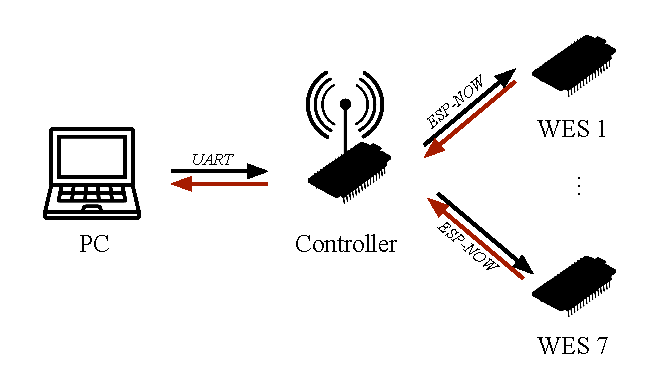
\includegraphics[scale=0.75]{figures/TestFlow.pdf}
	\caption{Data Flow for Measurement}
	\label{fig:testbed}
\end{figure}
\todo{change N to the actual number of WESs = 7}

The experiment is started from the PC, a JSON is then transmitted to the controller via \ac{UART} using a Python script.
The JSON contains all the parameters that are needed to carry out a test.
At the time the JSON string is transmitted, the controller should be idle so that the packet is read correctly.

\begin{table}[h]
	\centering
	\begin{tabular} { lll }
	\toprule
	\multicolumn{1}{c}{Variable}
	& \multicolumn{1}{c}{Example}
	& \multicolumn{1}{c}{Explaination} \\
	\midrule
	VERBOSE               & 0 				& Enable VERBOSE \\
	DEBUG                 & 0 				& Enable DEBUG \\
	TIMESTAMP\_UART       & 0				& Enable UART timestamps \\
	SEQUENCE\_REPITITIONS & 200				& Sequences per experiment \\
	FULL\_REPETITIONS     & 1000			& Repeations of the experiment \\
	MASTER\_CHANNEL       & 6				& Wifi Channel of the Controller \\
	WES\_CHANNEL          & 6				& Wifi Channel of the WES \\
	WAIT\_AFTER\_SEQ      & 0				& delay between sequences \\
	WAIT\_AFTER\_REP\_EXP & 2000			& delay between experiments \\
	IS\_BROADCASTING      & 1				& BC:=1, UC:=0 \\
	RAPID\_REPITITION     & 2				& BC: Rapid Repetitions \\
	CHANNEL\_TOTAL        & 160	 			& BC: Addressed Payload \\
	BROADCAST\_FRAME\_SIZE& 200 			& BC: Maximum Payload/Brodcast \\
	UNICAST\_FRAME\_SIZE  & 20				& UC: Payload/Unicast \\
	WES\_COUNT            & 6				& UC: WES Count \\
	AIRTIME               & 0				& Capture airtime\\
	\bottomrule
	\end{tabular}
	\caption{JSON Experiment Setup}
	\label{tab:json}
\end{table}

When the controller has received its JSON, it must go through three states, regardless of further input from the PC\cref{fig:sequenceDiagram}.
\subsubsection*{Setup}
After the start-up, the controller waits for a JSON. When the JSON is received, it sets the corresponding variables.
It then forwards these to the individual WESs using unicast. 
To be absolutely sure that the respective WES has received the setup information,
the number of retransmits in the application layer is set to infinity.
It distributes the data round robin, the MAC addresses of all WESs are hardcoded, but could also be transmitted via JSON.
If the first byte of the setup unicast is set to 253, the WES knows that it is a metadata packet and handles it accordingly in its callback.
\subsubsection*{Testing}
When the controller has ensured that each WES has received the measurement data, it starts transmitting the dummy test data.
Sequences are then sent according to the variable SEQUENCE\_REPETITIONS.
The duration varies greatly depending on the number of sequences and the protocol used.
\subsubsection*{Collecting}
When the controller has processed all sequences, it makes a request to one of the WESs, 
again with the help of a 100\% reliable unicast forced on the application layer.
This then transmits the measured values and in turn ensures that these have also arrived at the controller.
The measured values are then transmitted to the PC and the experiment is repeated until the required number of experiments has been completed.

\begin{figure}[h]
	\centering
	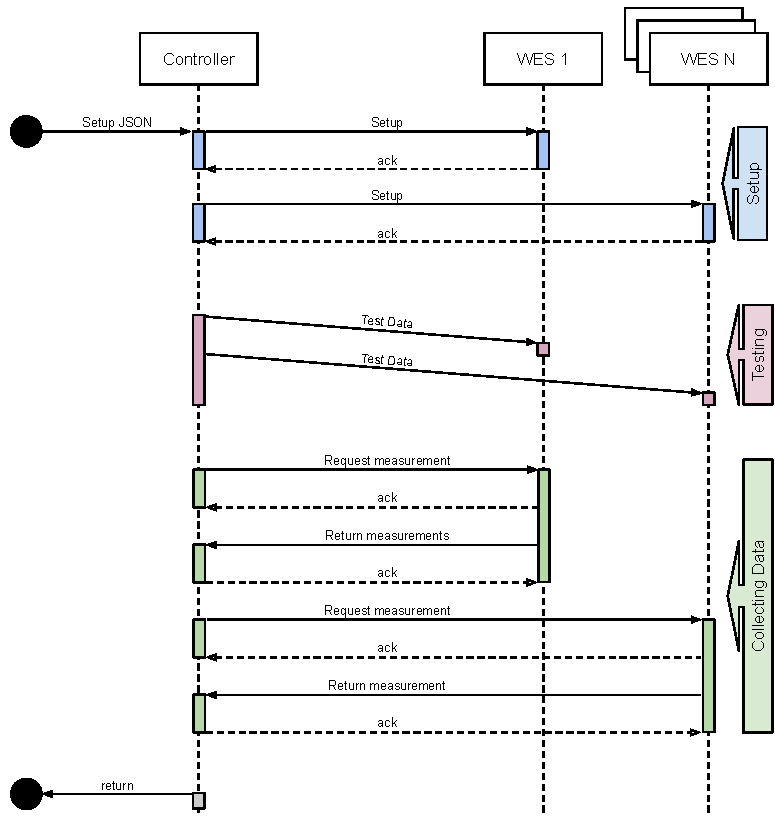
\includegraphics[scale=0.9]{figures/sequence_diagram_drive.pdf}
	\caption{Sequence Diagram of the Measurment}
	\label{fig:sequenceDiagram}
\end{figure}

\section{Wireshark measurements}

The Wireshark tool is suitable for recording traffic.
In order to record packets outside of a LAN, the WIFI card must be set to monitor mode.
In this mode, frames from an ad-hoc network can also be sniffed, as is the case with ESP-NOW.
In \cref{fig:wiresharkUC} it is clear to see that each unicast is followed by an acknolegement, as mentioned in the Chapter 3.

\begin{figure}[h]
	\centering
	\includegraphics[scale=0.5]{figures/wiresharkUC.pdf}
	\caption{Unicast Transmissions Recording from Wireshark}
	\label{fig:wiresharkUC}
\end{figure}

A look into the data frame \cref{fig:wiresharkUCTransmission} also shows the measured airtime of 696$\mu$s.
Adding the average backoff of a free channel (160$\mu$s) and the DIFS (50$\mu$s) gives 906$\mu$s.
In the calculation from \cref{tab:airtime_unicast_calc}, however, it was only 746$\mu$s.
\todo{TOLJA!\\yes.... actually why?}The difference of 120$\mu$s can be... 
Wireshark also recognises the category code of the Vendor Specific Action Frame that ESP-NOW uses.
The payload of 20 bytes assumed for unicast in the experiment is given here as 31 bytes,
presumably it has to do with the implementation of the action frame shown in \cref{fig:esp_now_vendor_format},
even though I can only figure out an offset of 10 bytes.\todo{is this personal note OK?}

\begin{figure}[h]
	\centering
	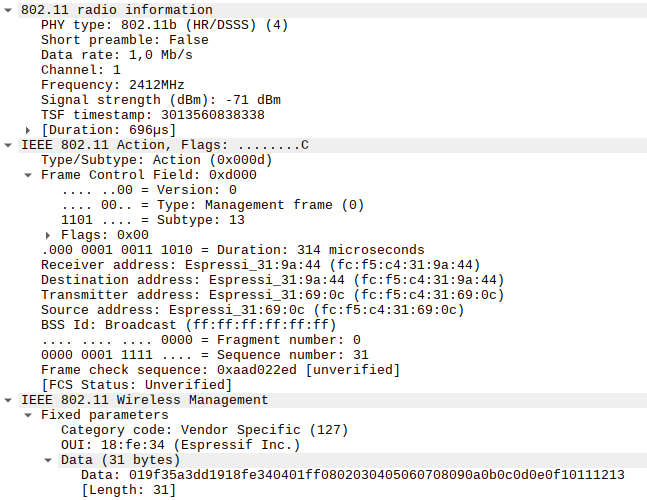
\includegraphics[scale=0.4]{figures/wiresharkUCFrame.png}
	\caption{Unicast Transmission Radio Information from Wireshark}
	\label{fig:wiresharkUCTransmission}
\end{figure}

\href{lst:callback}
A look at the 31 byte "payload" shows that ESP-NOW specific parts of wireshark have not been parsed correctly.
From the representation \cref{fig:esp-now_frame_format} and \cref{fig:esp-now_frame_format} it can be deduced:

that the first 4 bytes of the payload are still the random values and, according to Espressif, 
do not belong to the Vendor Specific Content.
These 4 bytes together with the following 1 byte (Element ID), 1 byte (length, interestingly specified as 25 Byte instead of 20),
Organisation Identifier (3 bytes), Type (1 byte) and Version (1 byte) make up the difference of 11 bytes to the actual payload.
\todo{This is barely readable}
The payload is filled with the flag ff \cref{lst:callback} followed by the sequence number, in this example 0.
The rest of the payload is filled with numbers, which are set to the value of the position in the payload.

\begin{figure}[h]
	\centering
	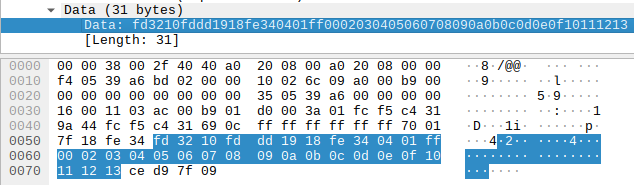
\includegraphics[scale=0.4]{figures/wiresharkPayload.png}
	\caption{Unicast Payload Analysis with Wireshark}
	\label{fig:wiresharkPayload}
\end{figure}

For completeness, here is a recording of the broadcast traffic.
The difference to the unicast traffic in \cref{wiresharkUCTransmission} is,
that the destination address is bundled in a transmission of 160 bytes instead of being distributed in 8x20 byte packets.
As already mentioned, the acknoledgments are not possible with the broadcast.

\begin{figure}[h]
	\centering
	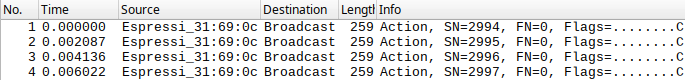
\includegraphics[scale=0.5]{figures/wiresharkBC.png}
	\caption{Unicast Payload Analysis with Wireshark}
	\label{fig:wiresharkBCTransmission}
\end{figure}

\section{Protocols under Study}

\subsection*{Slim Unicast vs Slim Broadcast}

\begin{figure}[h]
	\centering
	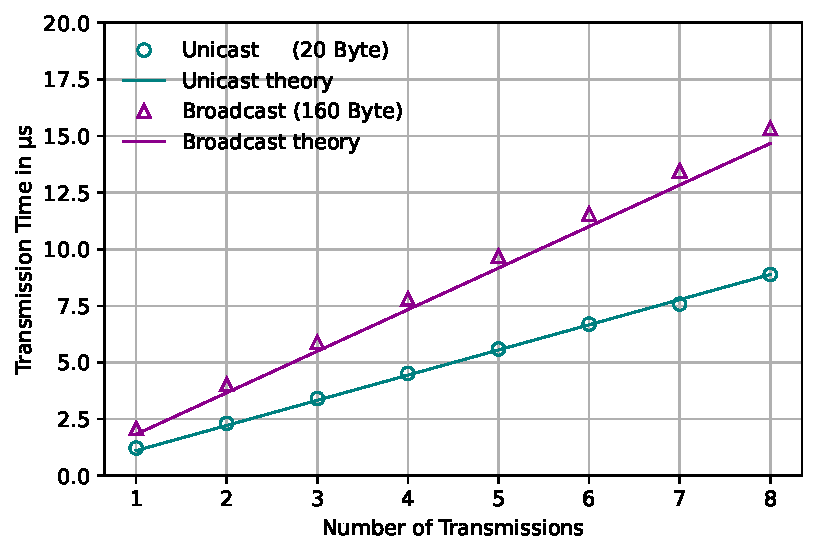
\includegraphics[scale=0.6]{../Plot2/Graphs/bc_uc_transmissiontime_wireshark.pdf}
	\caption{E.g. Transmission Time of Slim Unicast and Slim Broadcast}
	\label{fig:transmissionTime}
\end{figure}

\subsubsection{Latency}

\subsubsection{Reliability}

\todo{how to show 100\% success ratio?}

\begin{figure}[h]
	\centering
	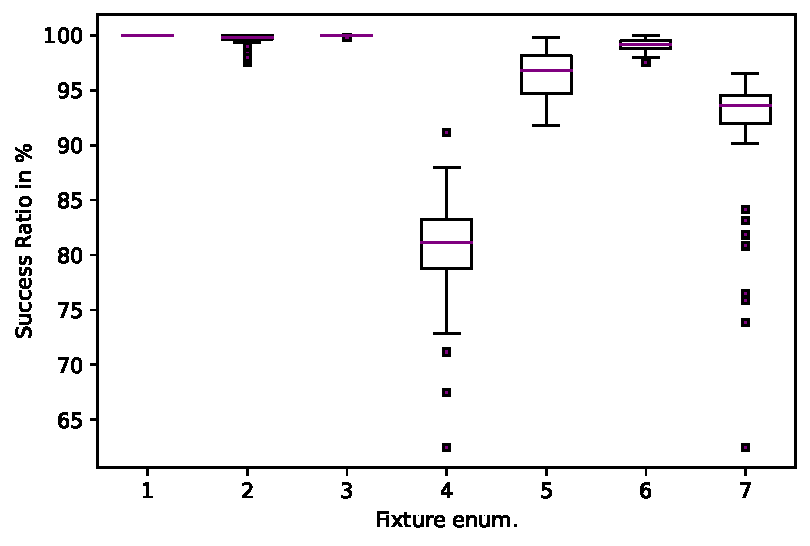
\includegraphics[scale=0.6]{../Plot2/Graphs/SR_per_fixture_broadcast.pdf}
	\caption{SR Broadcast}
	\label{fig:sr_broadcast}
\end{figure}

\subsection*{Rapid Repetition}

\begin{figure}[h]
	\centering
	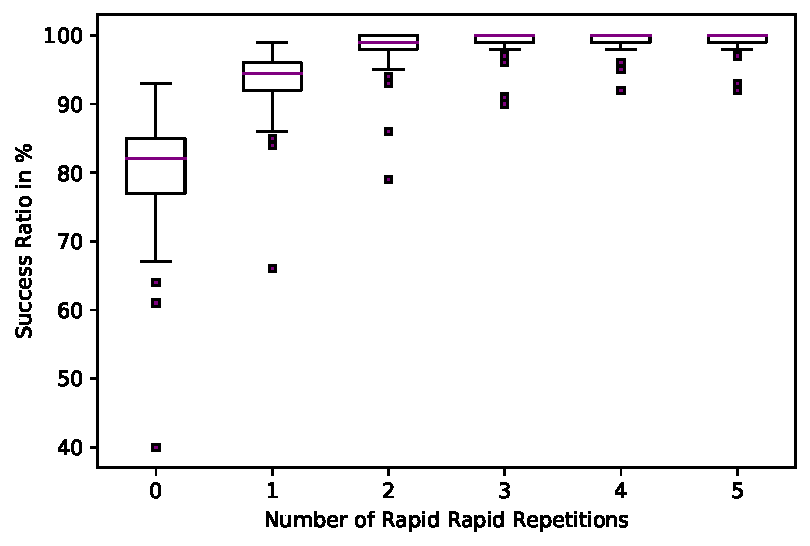
\includegraphics[scale=0.6]{../Plot2/Graphs/SR_of_node4_rr.pdf}
	\caption{SR of WES4 with altered RRs}
	\label{fig:sr_broadcast_wes4}
\end{figure}

\subsection*{Delayed Repetition}
\subsection*{Impact of Groupsize}

\section{Results}
\TODO{Difference between Results and Discussion?}
\begin{itemize}
	\item Grafen miteinander verlgeichen?
	\item Which method had the best results?
	\item Tabelle mit allen Protokollen auflisten 
\end{itemize}

\chapter{Conclusion \& Discussion}
\begin{itemize}
\item summarize again what your paper did, but now emphasize more the results, and comparisons
\item write conclusions that can be drawn from the results found and the discussion presented in the paper
\item future work (be very brief, explain what, but not much how, do not speculate about results or impact)
\item recommended length: one page.
\end{itemize}

Why not 5GHz -> to expensive.\\


\section*{Keep in Mind}
\begin{itemize}
\item metrics (SR, Latency, ...)
\item compare with art-net all the time
\item wireshark
\end{itemize}